\noindent
Cuando proyectamos una escena del mundo real en tres dimensiones sobre un plano bidimensional, como la película o el sensor de una cámara, se produce una transformación en la imagen.
Esta transformación, conocida como transformación proyectiva, provoca que las líneas paralelas en el mundo real, al proyectarse en el plano de la cámara, se intersecten en un punto denominado punto de fuga.

\begin{figure}[!ht]
    \centering
    \begin{subfigure}{0.4\textwidth}
        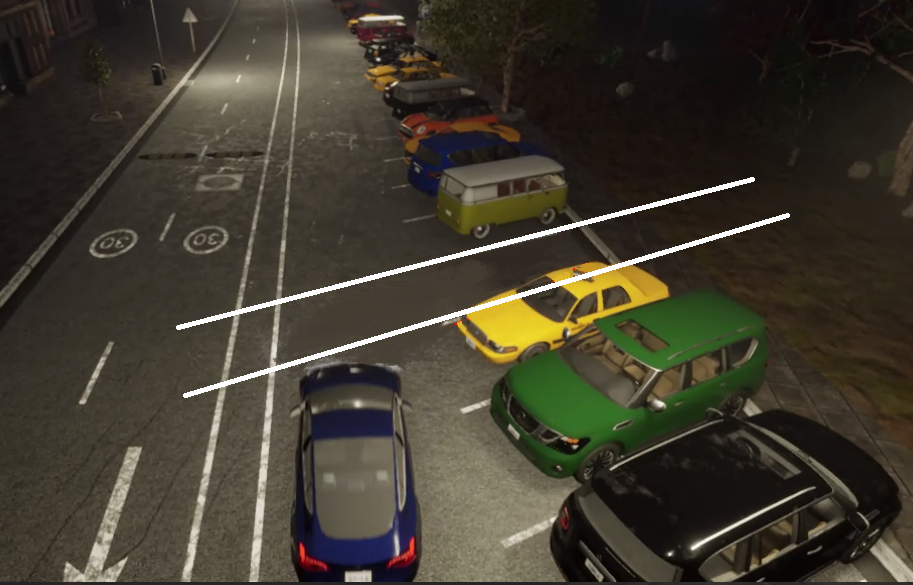
\includegraphics[width=\textwidth]{img/reticule/paralel_lines}\label{fig:parallel_lines}
        \caption{Ejemplo de líneas paralelas en un escenario real en tres dimensiones.}
    \end{subfigure}
    \begin{subfigure}{0.4\textwidth}
        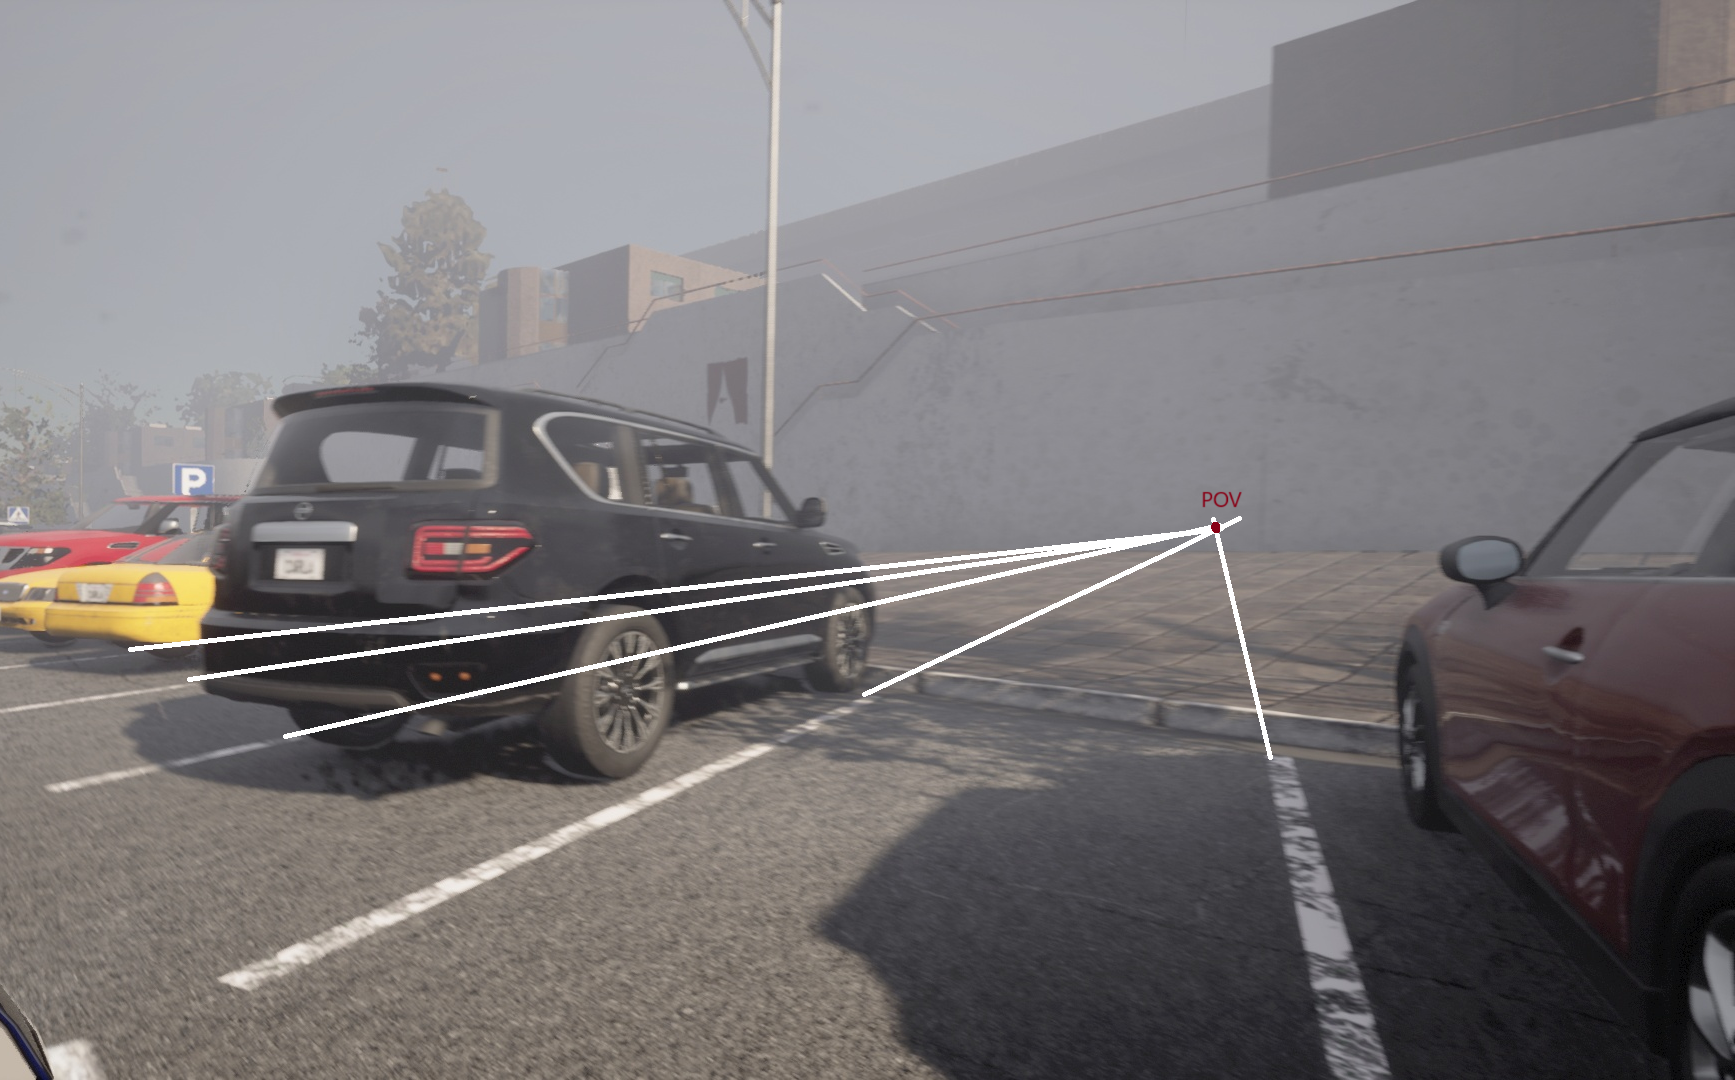
\includegraphics[width=\textwidth]{img/reticule/pov}\label{fig:pov}
        \caption{Proyección de líneas paralelas en el plano de la cámara.}
    \end{subfigure}

    \label{fig:distorion}
\end{figure}

\noindent
Dado que las líneas de los cajones de estacionamiento son paralelas por su geometría, forman patrones en una retícula de paralelogramos.
Esto permite utilizar técnicas de detección de líneas para identificar los puntos de fuga y estimar la posición de la retícula de estacionamiento.
En la figura \ref{fig:reticule_pov} se muestra un ejemplo de la retícula de estacionamiento vista desde la perspectiva de la cámara del vehículo.

\begin{figure}[!ht]
    \centering
    \begin{subfigure}{0.8\textwidth}
        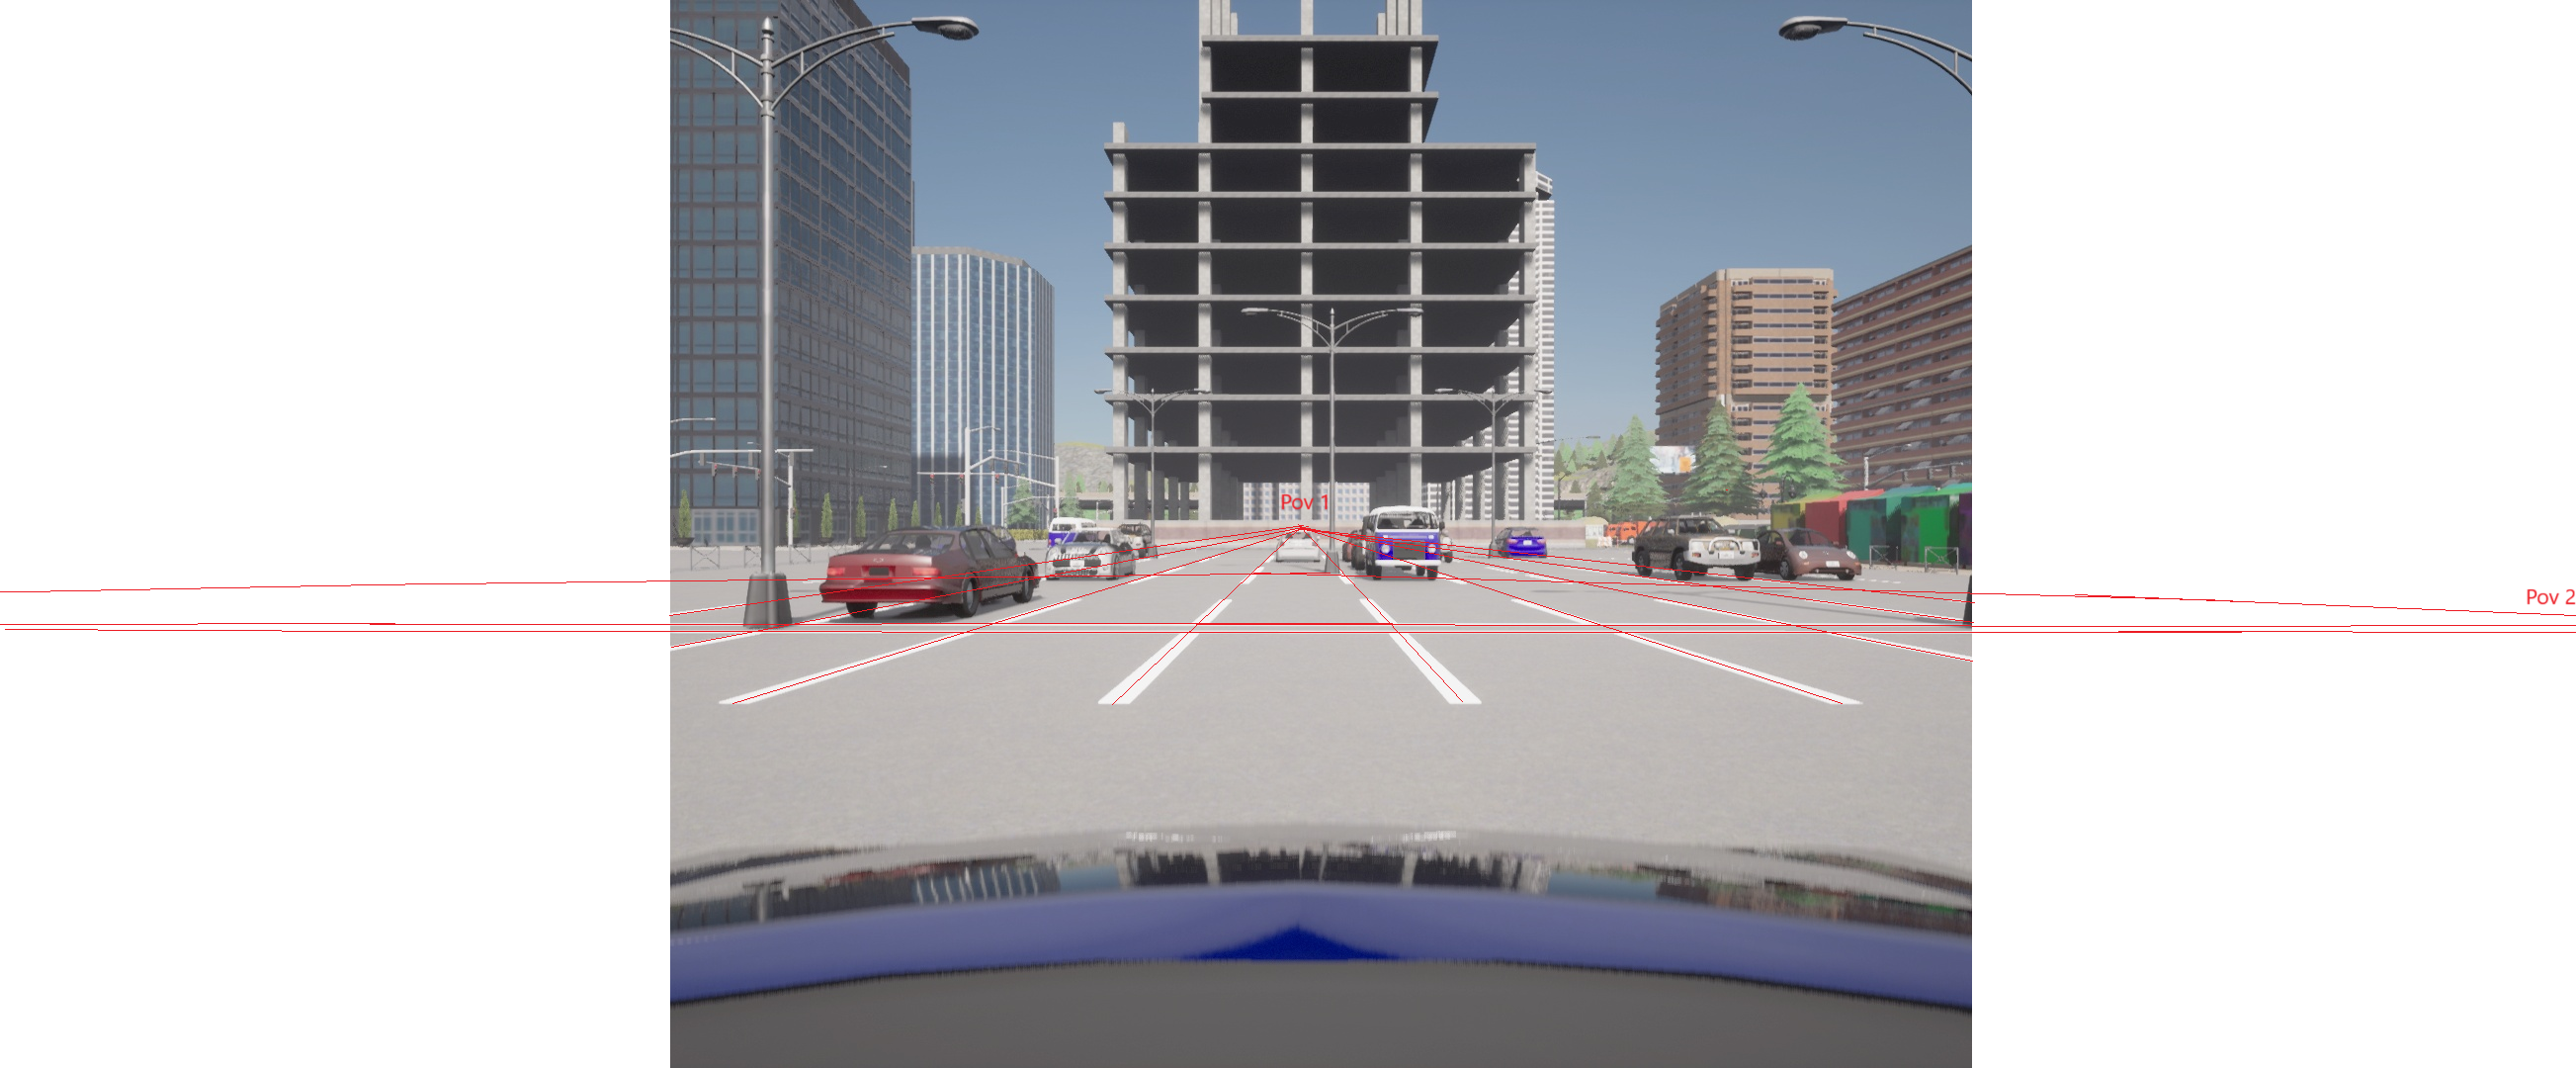
\includegraphics[width=\textwidth]{img/reticule/pov_reticule}\label{fig:pov_reticule}
    \end{subfigure}
    \begin{subfigure}{0.8\textwidth}
        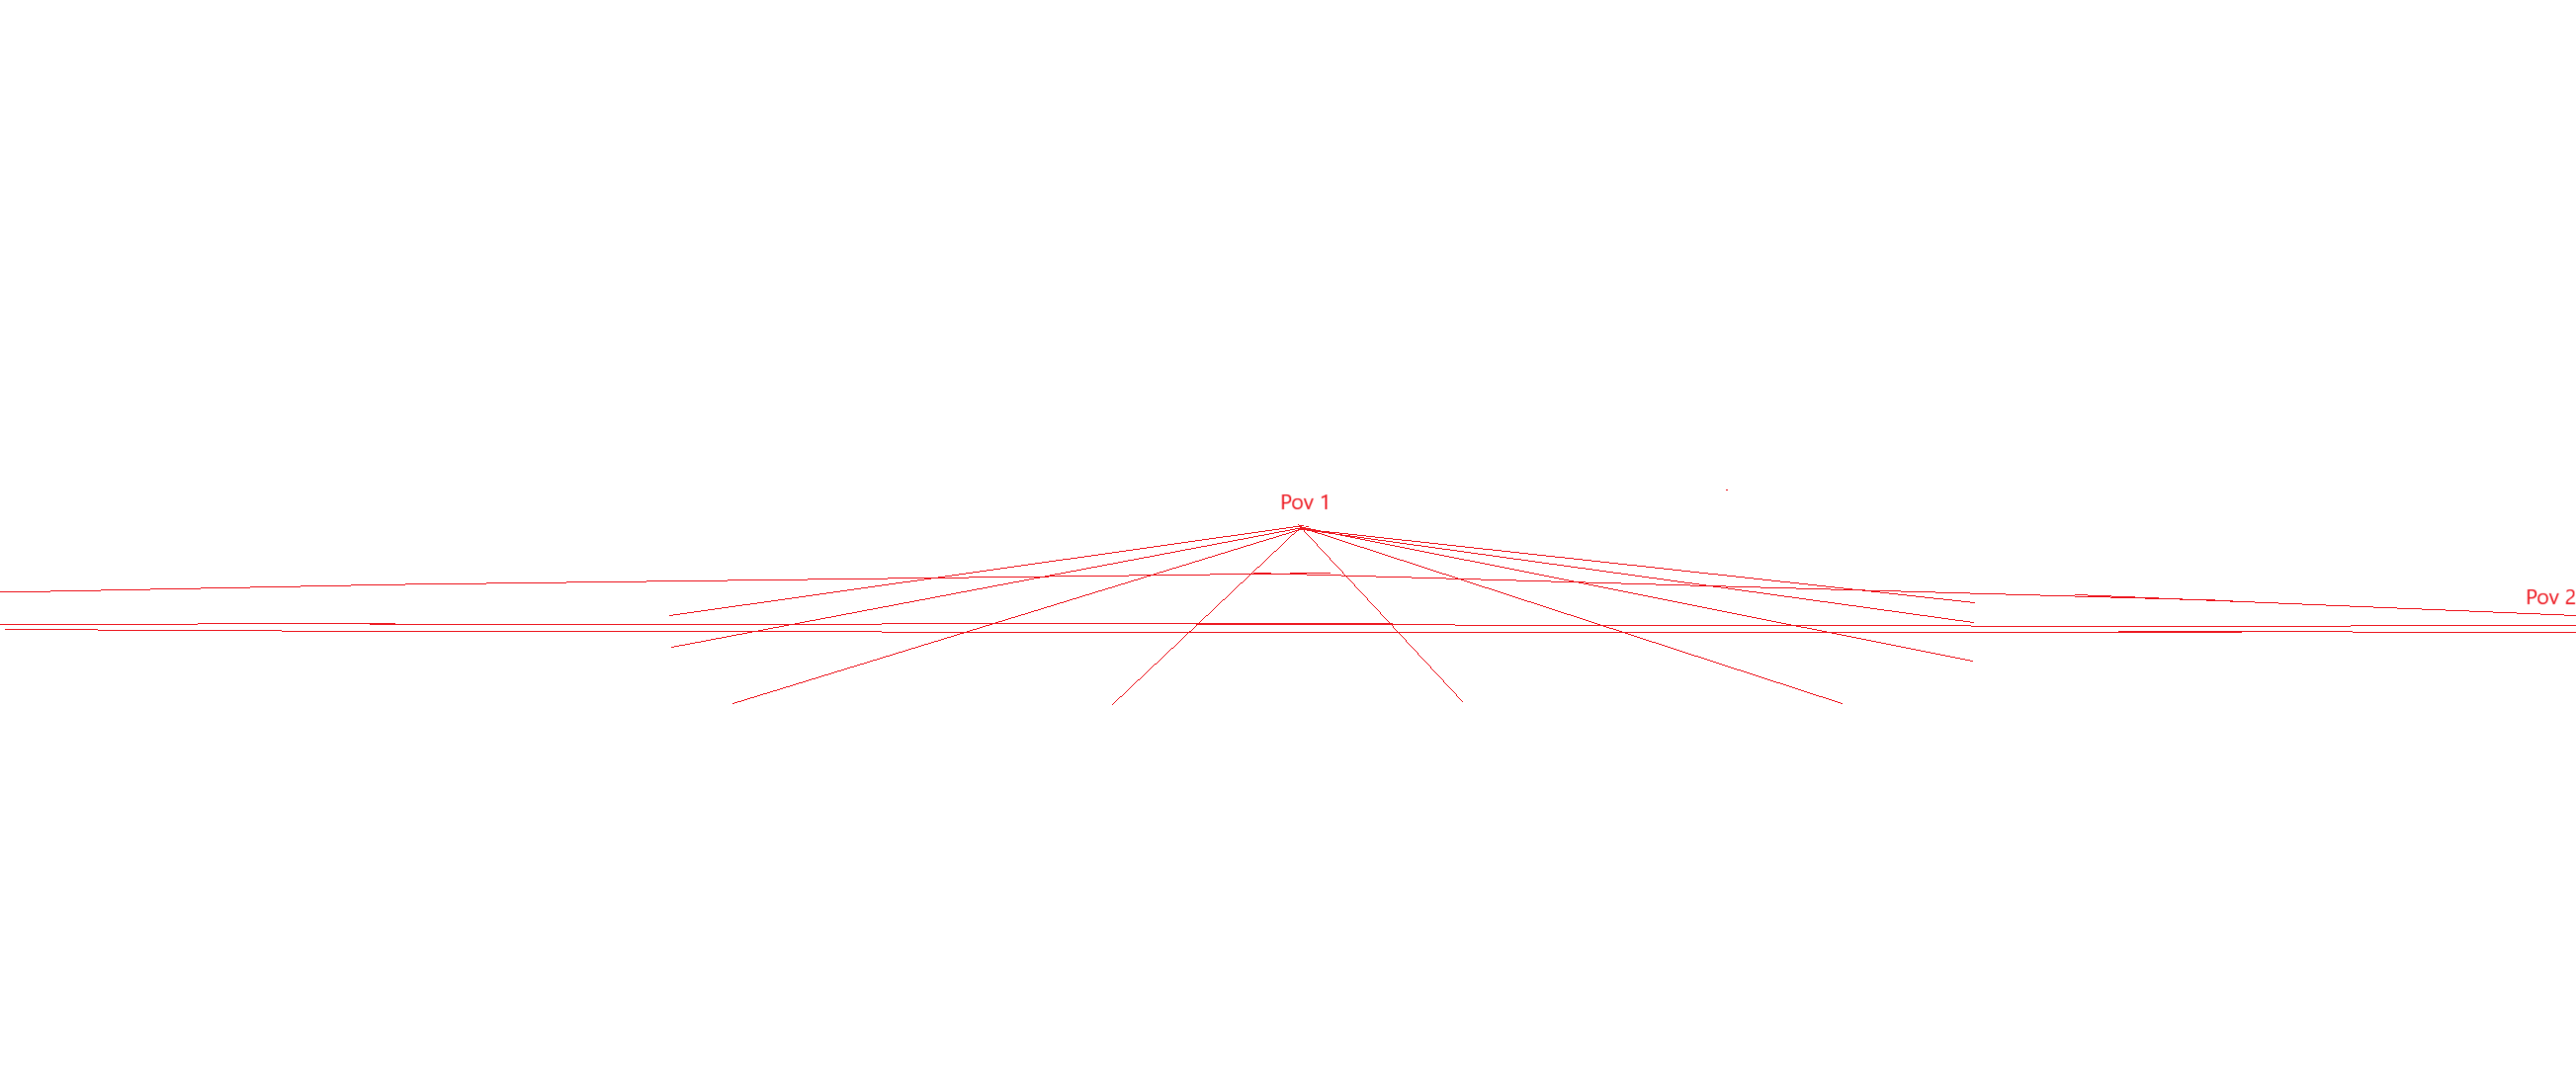
\includegraphics[width=\textwidth]{img/reticule/pov_reticule_layer}\label{fig:pov_reticule_layers}
    \end{subfigure}
    \caption{Líneas paralelas de la retícula de estacionamiento.}
    \label{fig:reticule_pov}
\end{figure}

\noindent
En esta sección se describen los pasos prácticos para identificar y analizar las líneas paralelas presentes en la imagen,
esenciales para la estimación de la retícula de estacionamiento.
El enfoque se centra en el procesamiento de la imagen y la extracción de información geométrica relevante,
utilizando técnicas clásicas de visión computacional.


\subsubsection{Área de interés:}
\noindent
Teniendo en cuenta que la cámara del vehículo se encuentra ubicada en la parte delantera a una altura conocida y en un ángulo paralelo al suelo, el área de interés de la imagen donde se encuentran las líneas de los cajones de estacionamiento quedará siempre por debajo del horizonte de la imagen.
Por lo tanto, se puede eliminar la parte superior de la imagen para
reducir el ruido y mejorar la detección de las líneas, como se muestra en la figura \ref{fig:roi}. \\
\begin{figure}[!ht]
    \centering
    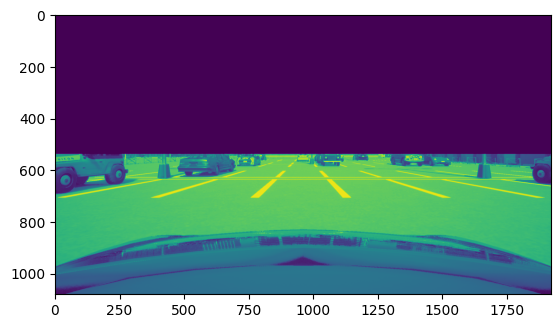
\includegraphics[width=0.8\textwidth]{img/reticule/horizont}
    \caption{Área de interés de la imagen}
    \label{fig:roi}
\end{figure}

\subsubsection{Umbralización:}
\noindent
Al área de interés de la imagen se le aplica una umbralización para realzar las líneas blancas de los cajones de estacionamiento
y eliminar otros elementos no relevantes que puedan interferir en la detección.
En la figura \ref{fig:threshold} se muestra un ejemplo de la imagen umbralizada.
\begin{figure}[!ht]
    \centering
    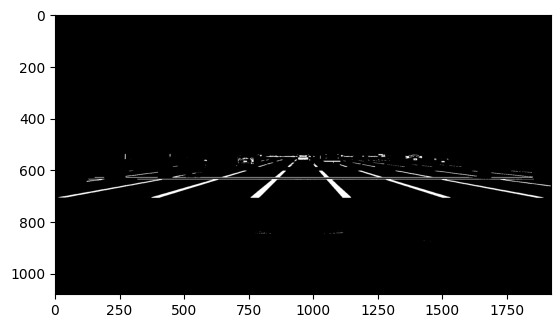
\includegraphics[width=0.8\textwidth]{img/reticule/thresholded}
    \caption{Imagen umbralizada}
    \label{fig:threshold}
\end{figure}

\subsubsection{Detección de contornos (Canny):}
\noindent
Se utiliza el algoritmo de Canny \cite{canny1986edge} para detectar los bordes de las líneas en la imagen umbralizada.
En la figura \ref{fig:edges} se muestra un ejemplo de la imagen con los bordes detectados.
\begin{figure}[!ht]
    \centering
    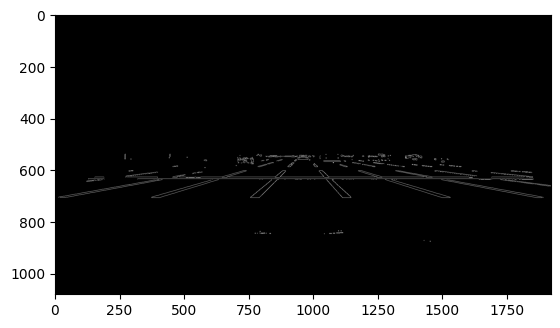
\includegraphics[width=0.6  \textwidth]{img/reticule/canny}
    \caption{Detección de bordes mediante el algoritmo de Canny}
    \label{fig:edges}
\end{figure}

\subsubsection{Detección de líneas (Hough):}
\noindent
Se aplica la transformada de Hough \cite{ballard1981hough} para detectar las coordenadas de inicio y fin de las líneas en la imagen.
En las figuras \ref{fig:hough} y \ref{fig:lines} se muestran las líneas detectadas sin fondo y sobre la imagen original, respectivamente.
\begin{figure}[!ht]
    \begin{subfigure}{0.5\textwidth}
        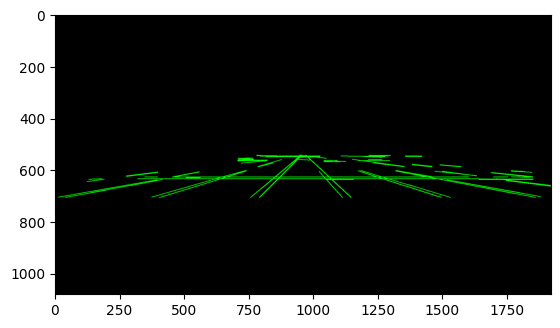
\includegraphics[width=\textwidth]{img/reticule/hough2}
        \caption{Líneas detectadas con la transformada de Hough}
        \label{fig:hough}
    \end{subfigure}
    \begin{subfigure}{0.5\textwidth}
        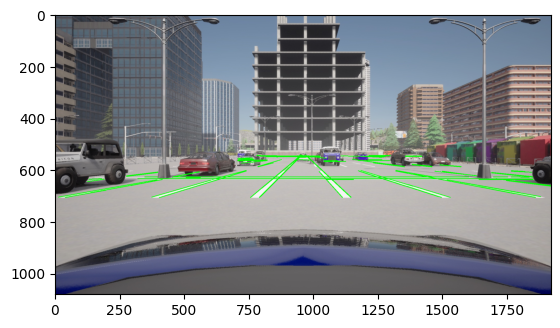
\includegraphics[width=\textwidth]{img/reticule/hough}
        \caption{Líneas detectadas en la imagen original}
        \label{fig:lines}
    \end{subfigure}
\end{figure}

\subsubsection{Representación de las ecuaciones de las líneas:}
\noindent
Una vez obtenidas las coordenadas de inicio y fin de cada línea paralela, se puede utilizar la ecuación general de la recta:
\begin{equation}
    Ax + By + C = 0
\end{equation}
Esta ecuación permite determinar la orientación de cada línea.
Dado que las coordenadas iniciales y finales de cada línea corresponden a los valores de $x$ y $y$, respectivamente,
estas se pueden emplear para formular un sistema de ecuaciones que describa los parámetros de la recta $[A, B, C]$.
Dicho sistema puede representarse de manera matricial como sigue:
\begin{equation}
    \begin{aligned}
        \left[\begin{array}{ccc}
                      x_1 & y_1 & 1 \\
                      x_2 & y_2 & 1
                  \end{array}\right]
        \begin{bmatrix}
            A \\
            B \\
            C
        \end{bmatrix}
        =
        \begin{bmatrix}
            0 \\
            0
        \end{bmatrix}
    \end{aligned}
\end{equation}

Esta representación permite calcular de forma precisa los coeficientes de la ecuación de la recta para cada línea detectada,
lo cual es fundamental para analizar su orientación y posición dentro de la retícula de estacionamiento.

\subsubsection{Cálculo de ecuaciones de las líneas (SVD):}
\noindent
Para calcular los coeficientes $[A, B, C]$ de las ecuaciones de las líneas detectadas, se utiliza el concepto de espacio nulo (\emph{null space}).
Este enfoque se basa en el hecho de que cualquier vector en el espacio nulo de una matriz $\mathbf{M}$ satisface la ecuación
\begin{equation}
    \mathbf{Mv} = 0
\end{equation}

%Comentario: No has definido el vector v.


Cada línea se representa mediante dos puntos $(x_1, y_1)$ y $(x_2, y_2)$. A partir de estas coordenadas homogéneas,
se construye una matriz $\mathbf{M}$ de la forma:
\[
    \mathbf{M} = \begin{bmatrix}
        x_1 & y_1 & 1 \\
        x_2 & y_2 & 1
    \end{bmatrix}
\]
Esta matriz define el sistema de ecuaciones que describe la recta que pasa por los puntos dados.
El espacio nulo de $\mathbf{M}$ corresponde al conjunto de vectores $[A,B,C]$ que satisfacen
\[
    \mathbf{M} \cdot \begin{bmatrix}
        A \\ B \\ C
    \end{bmatrix} = \mathbf{0}.
\]
Se utiliza la Descomposición en Valores Singulares (SVD) \cite{golub2013matrix} para calcular este espacio nulo, ya que es una herramienta robusta y numéricamente estable.
La SVD descompone la matriz \(M\) en tres matrices \(U\), \(S\) y \(V\), donde el espacio nulo de \(M\) se puede obtener a partir de la última columna de la matriz \(V\), que corresponde al vector singular más pequeño (el más cercano a cero).
El vector resultante del espacio nulo se normaliza para que tenga una magnitud manejable.
Esto asegura que los coeficientes \(A\), \(B\) y \(C\) sean comparables entre distintas líneas.

\subsubsection{Cálculo de intersecciones (Clustering):}
\noindent
Una vez que se tienen las ecuaciones de todas las líneas paralelas en el plano de la cámara, se pueden calcular las intersecciones de estas líneas realizando un producto cruz entre las ecuaciones homogéneas [\(A\),\(B\),\(C\)] de todos los pares de líneas.

El resultado de este producto cruz es la coordenada homogénea de un punto en el espacio que corresponde a la intersección de las líneas.
Si este punto es finito (cuando la tercera componente no es cero), se puede deshomogeneizar para obtener las coordenadas cartesianas en el plano de la cámara.
En cambio, si el punto es infinito (cuando la tercera componente es muy cercana a cero), significa que las líneas son paralelas y se intersectan en el infinito.


\textit{Agrupación de intersecciones:}
%https://scikit-learn.org/stable/modules/clustering.html#hierarchical-clustering

Analizando los puntos de intersección obtenidos que se encuentran en el plano de la cámara, se pueden agrupar para determinar dónde está
concentrada la mayor cantidad de intersecciones.
Este punto de concentración de intersecciones debe corresponder al punto de fuga principal de la retícula de estacionamiento.
En la figura \ref{fig:intersections} se muestra un ejemplo de las intersecciones detectadas en la imagen original,
donde cada color representa un cluster diferente y el símbolo \texttt{+} blanco indica el centro de cada cluster.
\\

\begin{figure}[!ht]
    \centering
    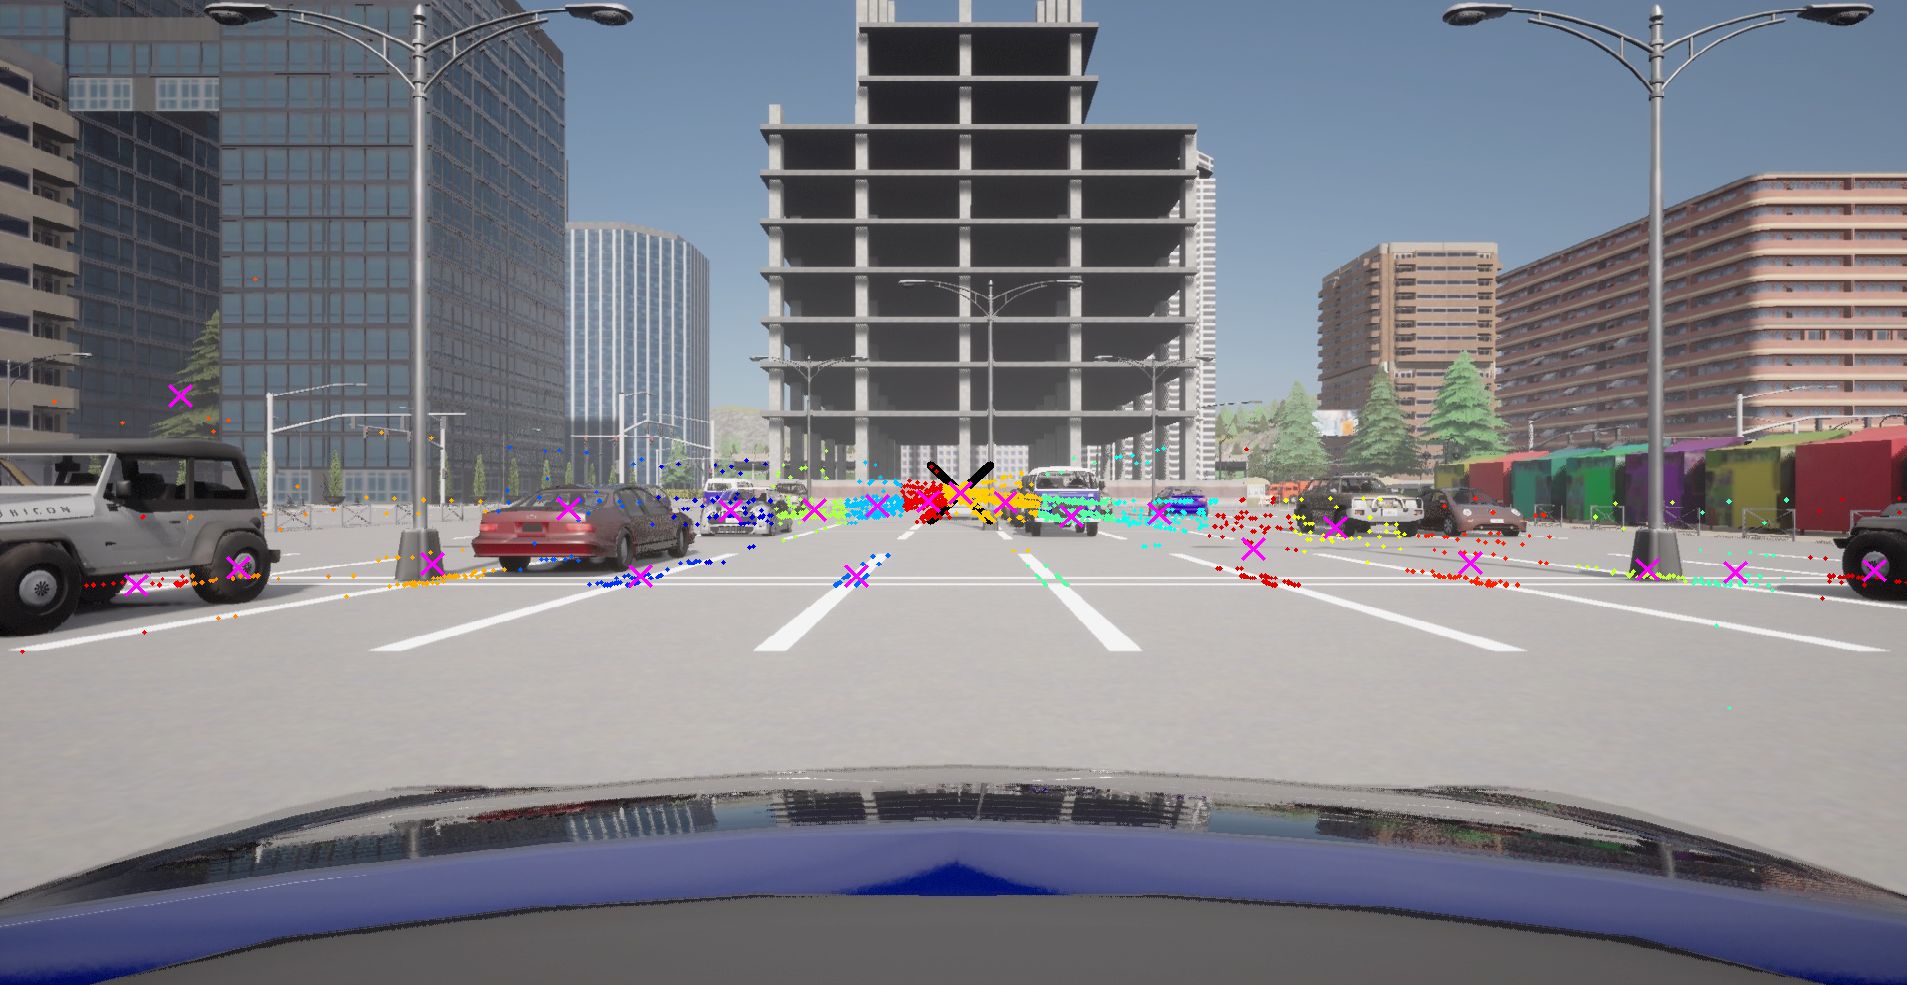
\includegraphics[width=0.8\textwidth]{img/reticule/svd-km}
    \caption{Agrupacion de intersecciones de las líneas detectadas}
    \label{fig:intersections}
\end{figure}

Para estimar la ubicación de este punto de fuga principal no es necesario tener en cuenta todas las intersecciones detectadas,
sino solo aquellas que se encuentran en una zona cercana al horizonte de la imagen.
Esto se debe a que, debido a la perspectiva de la cámara, las líneas paralelas en el mundo real convergen hacia el horizonte en la imagen,
haciendo que los puntos de fuga se ubiquen cerca de esta línea \cite{hartley2003multiple}.
Para determinar las intersecciones relevantes cercanas al horizonte, se puede definir un umbral de cercanía en la imagen que se puede ajustar experimentalmente.
Por ejemplo, en la siguiente imagen se muestran las intersecciones detectadas en la imagen original con puntos azules
y las intersecciones relevantes con un umbral de 10 píxeles con puntos amarillos.
En la figura \ref{fig:relevantInter} se muestra el resultado de la selección de las intersecciones relevantes. \\
\begin{figure}[!ht]
    \centering
    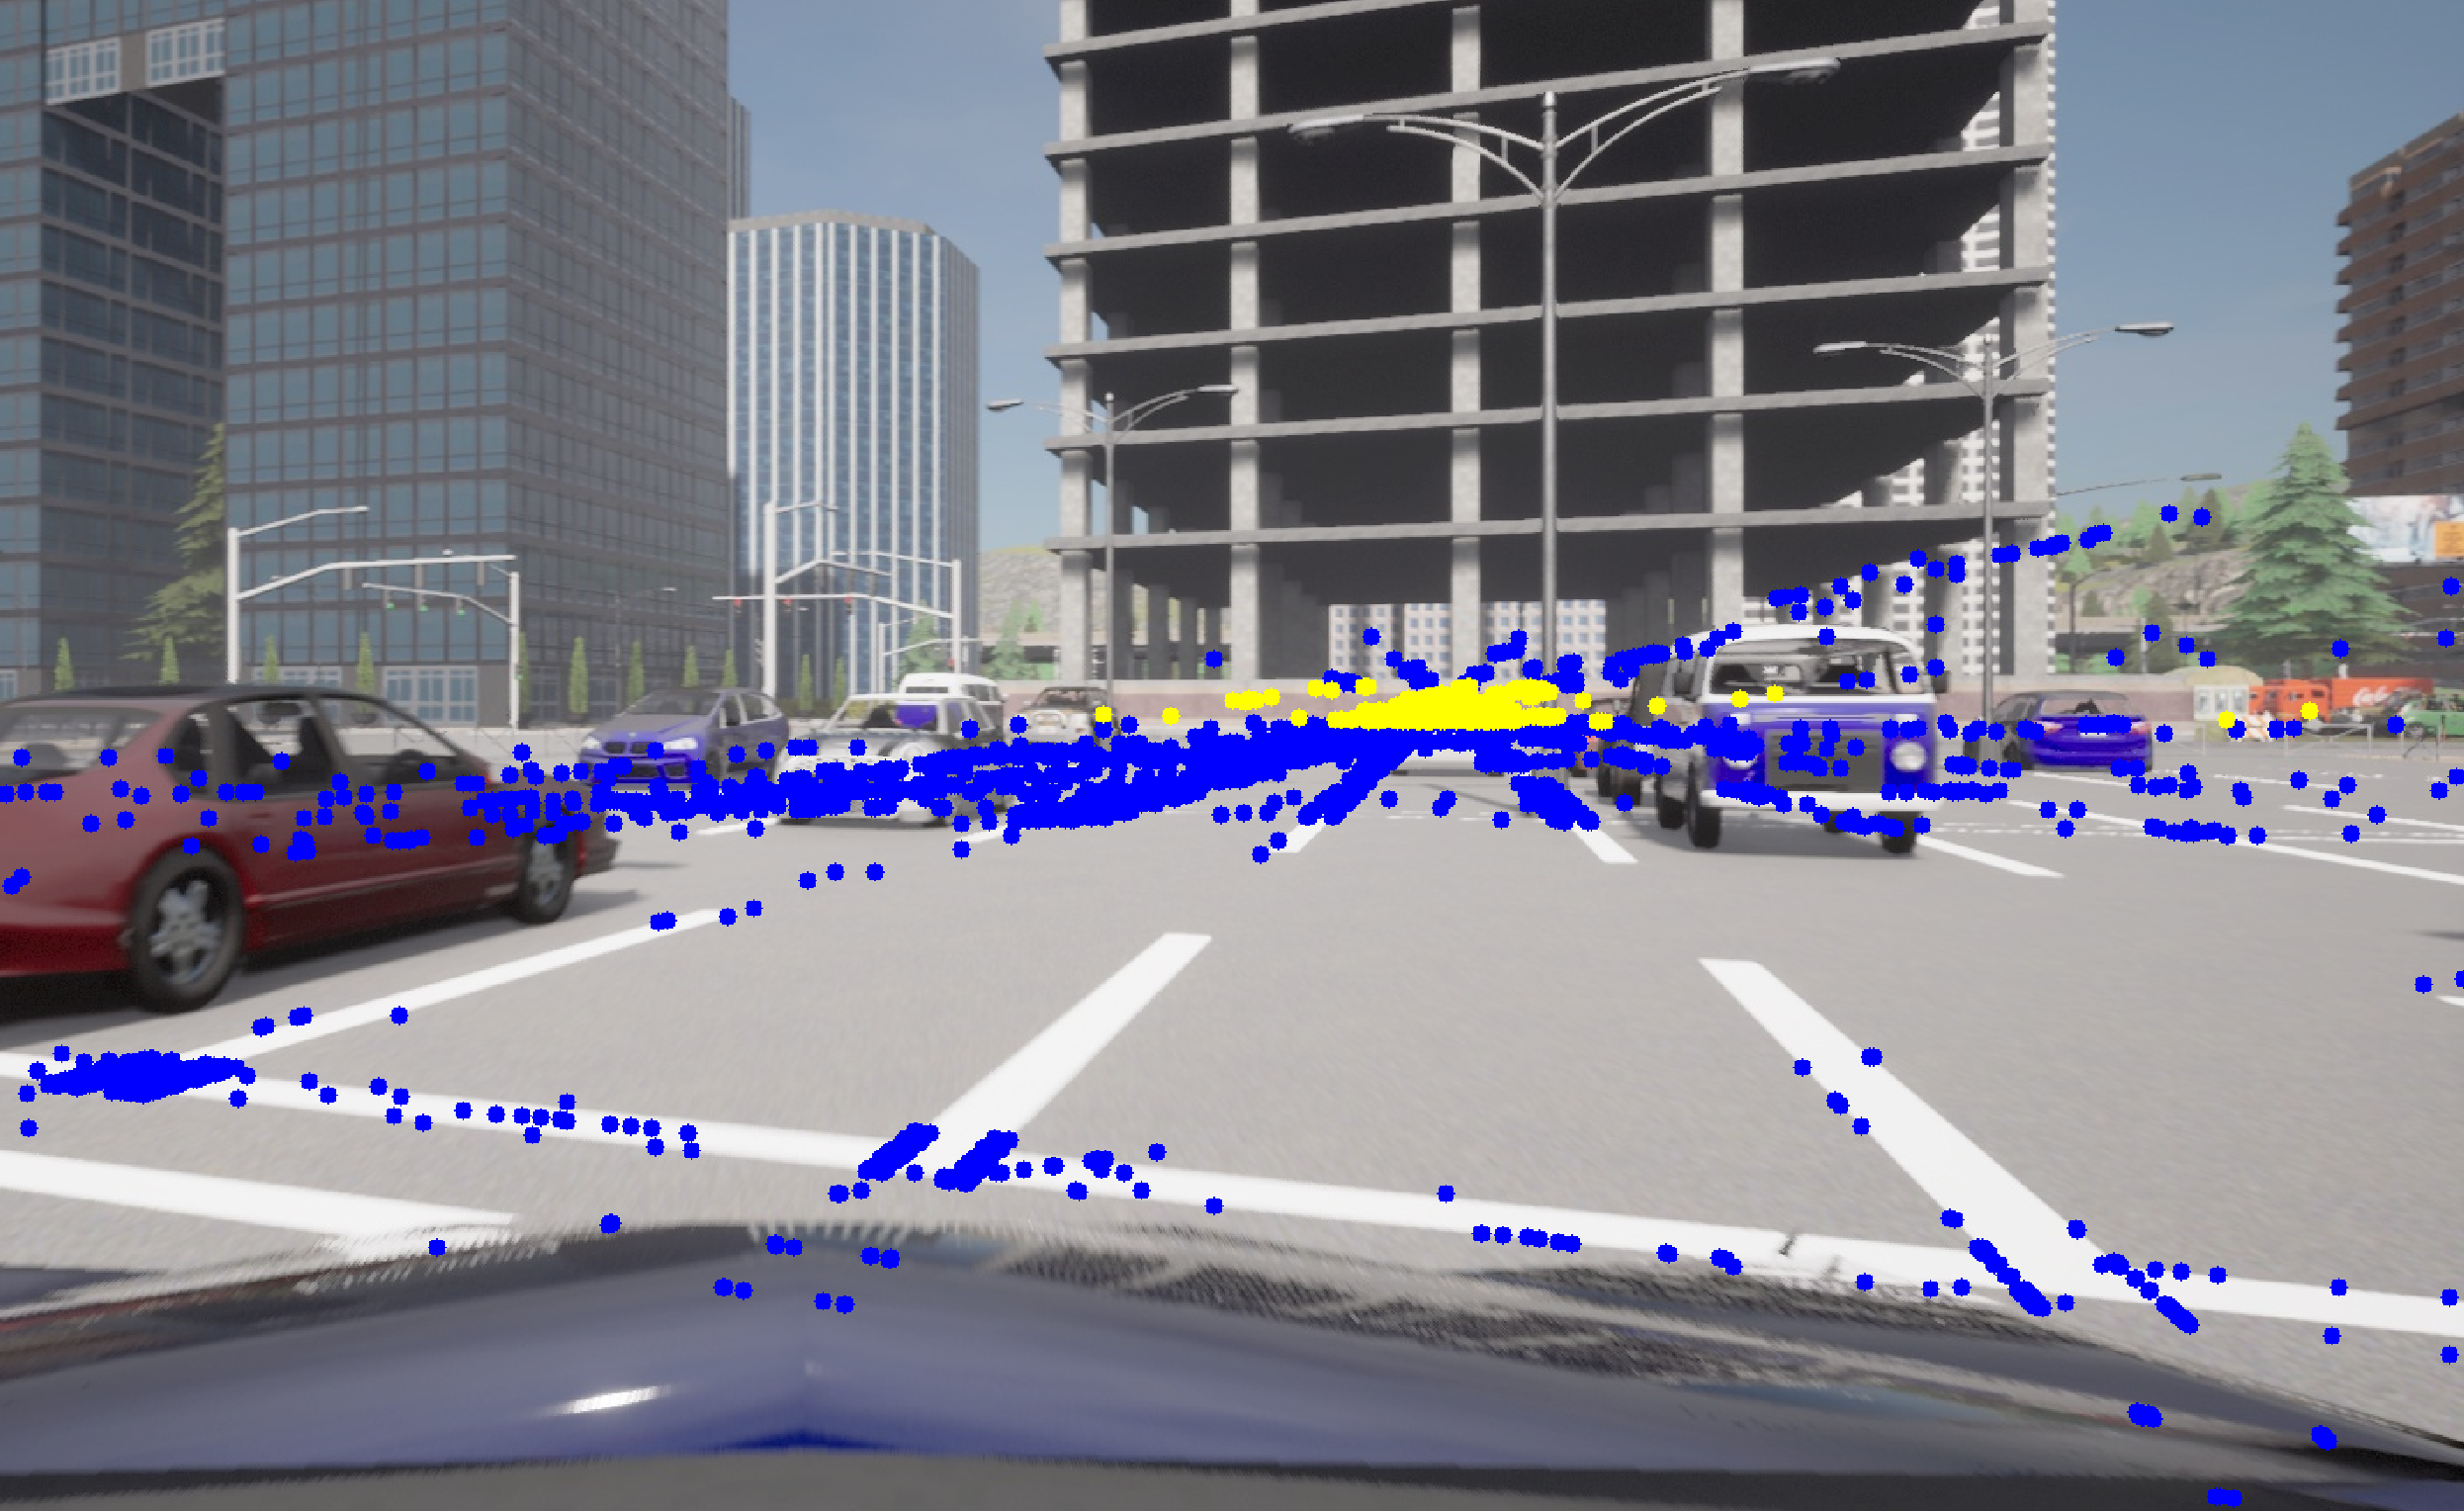
\includegraphics[width=0.8\textwidth]{img/reticule/relevantInter}
    \caption{Intersecciones detectadas en la imagen original}
    \label{fig:relevantInter}
\end{figure}

\textit{Algoritmo de agrupación:}\\

Para realizar la agrupación de las intersecciones relevantes, se utilizó el algoritmo \texttt{AgglomerativeClustering} de la librería \texttt{scikit-learn}.
Este algoritmo fue elegido debido a su capacidad para manejar datos jerárquicos y su flexibilidad para determinar el número óptimo de clusters. Además,
es robusto frente a la variabilidad en la densidad de los puntos de intersección.
El algoritmo de agrupación jerárquica se basa en la idea de que los puntos cercanos entre sí pertenecen al mismo cluster \cite{tan2005introduction}.
Para que el algoritmo determine el número de clusters se utilizó el parámetro \texttt{distance\_threshold}, que indica la distancia máxima
entre dos puntos para que se consideren en el mismo cluster. El valor de este parámetro se puede ajustar experimentalmente.
Por ejemplo, en la siguiente imagen se muestran los mismos puntos de intersección relevantes del ejemplo anterior,
pero agrupados por el algoritmo de agrupación jerárquica en 3 clusters representados de distintos colores, con un símbolo \texttt{+} blanco en el centro de cada cluster.
En la figura \ref{fig:clusters} se muestra el resultado de la agrupación de las intersecciones relevantes.
\begin{figure}[!ht]
    \centering
    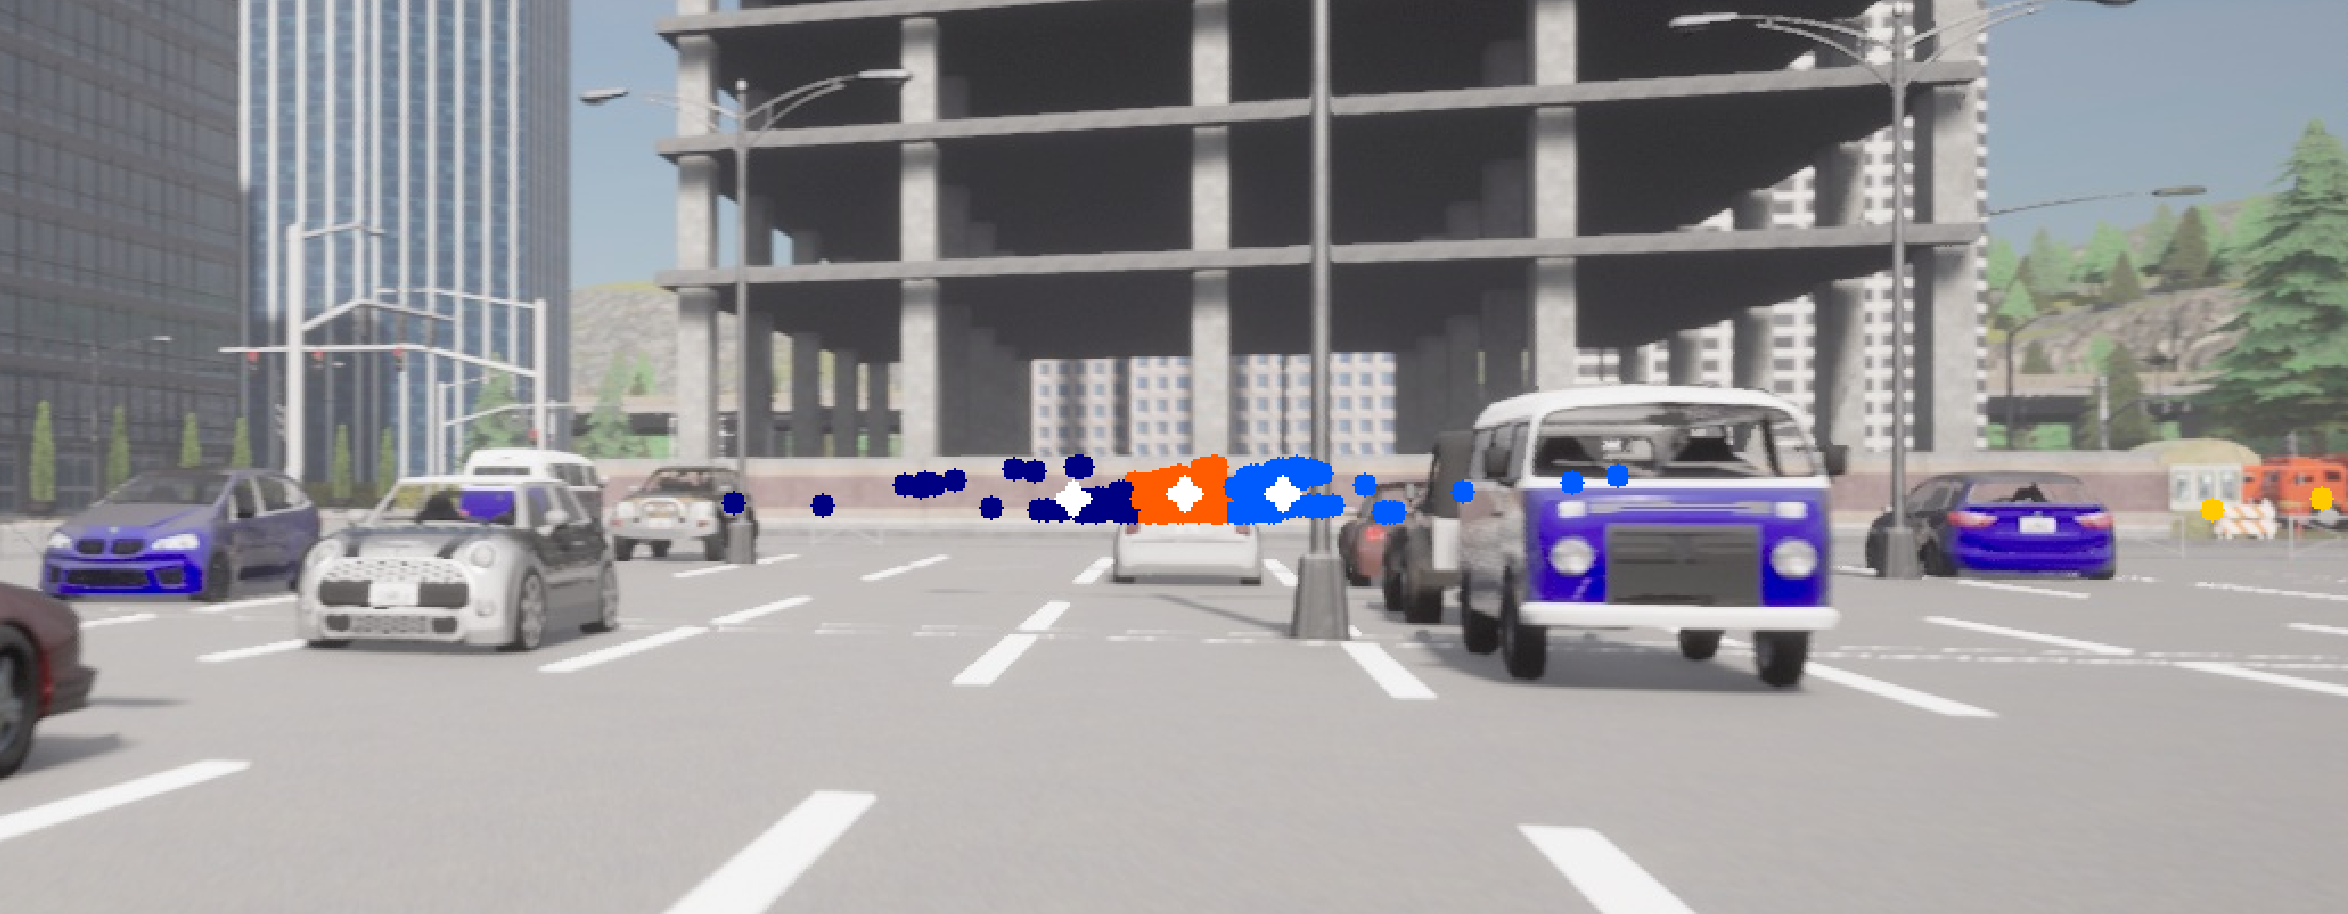
\includegraphics[width=0.8\textwidth]{img/reticule/AgglomerativeClustering}
    \caption{Intersecciones agrupadas en clusters}
    \label{fig:clusters}
\end{figure}



\subsubsection{Selección del punto de fuga principal:}
\noindent
Para estimar la posición del punto de fuga principal, se puede seleccionar el cluster con mayor cantidad de intersecciones y
utilizar las líneas que generaron estos puntos para calcular la intersección de estas líneas.
La intersección de $n$ líneas (bajo un criterio de mínimos cuadrados) está dada por
el eigenvector asociado al eigenvalor más pequeño de la matriz $M$, donde:
\[
    M = \sum_{i=1}^{n} w_i l_i l_i^T
\]
Aquí, $w_i$ es un peso asociado a la línea $l_i$ y $l_i$ es la representación homogénea de la línea $i$ \cite{kanatani1998statistical}.
De esta forma, podemos conocer la posición del punto de fuga principal en el plano de la cámara.
En la figura \ref{fig:vanishingPoint} se muestra el resultado de esta estimación utilizando las líneas del cluster más grande, donde se
representa el punto de fuga principal con un símbolo \texttt{+} amarillo.
\begin{figure}[!ht]
    \centering
    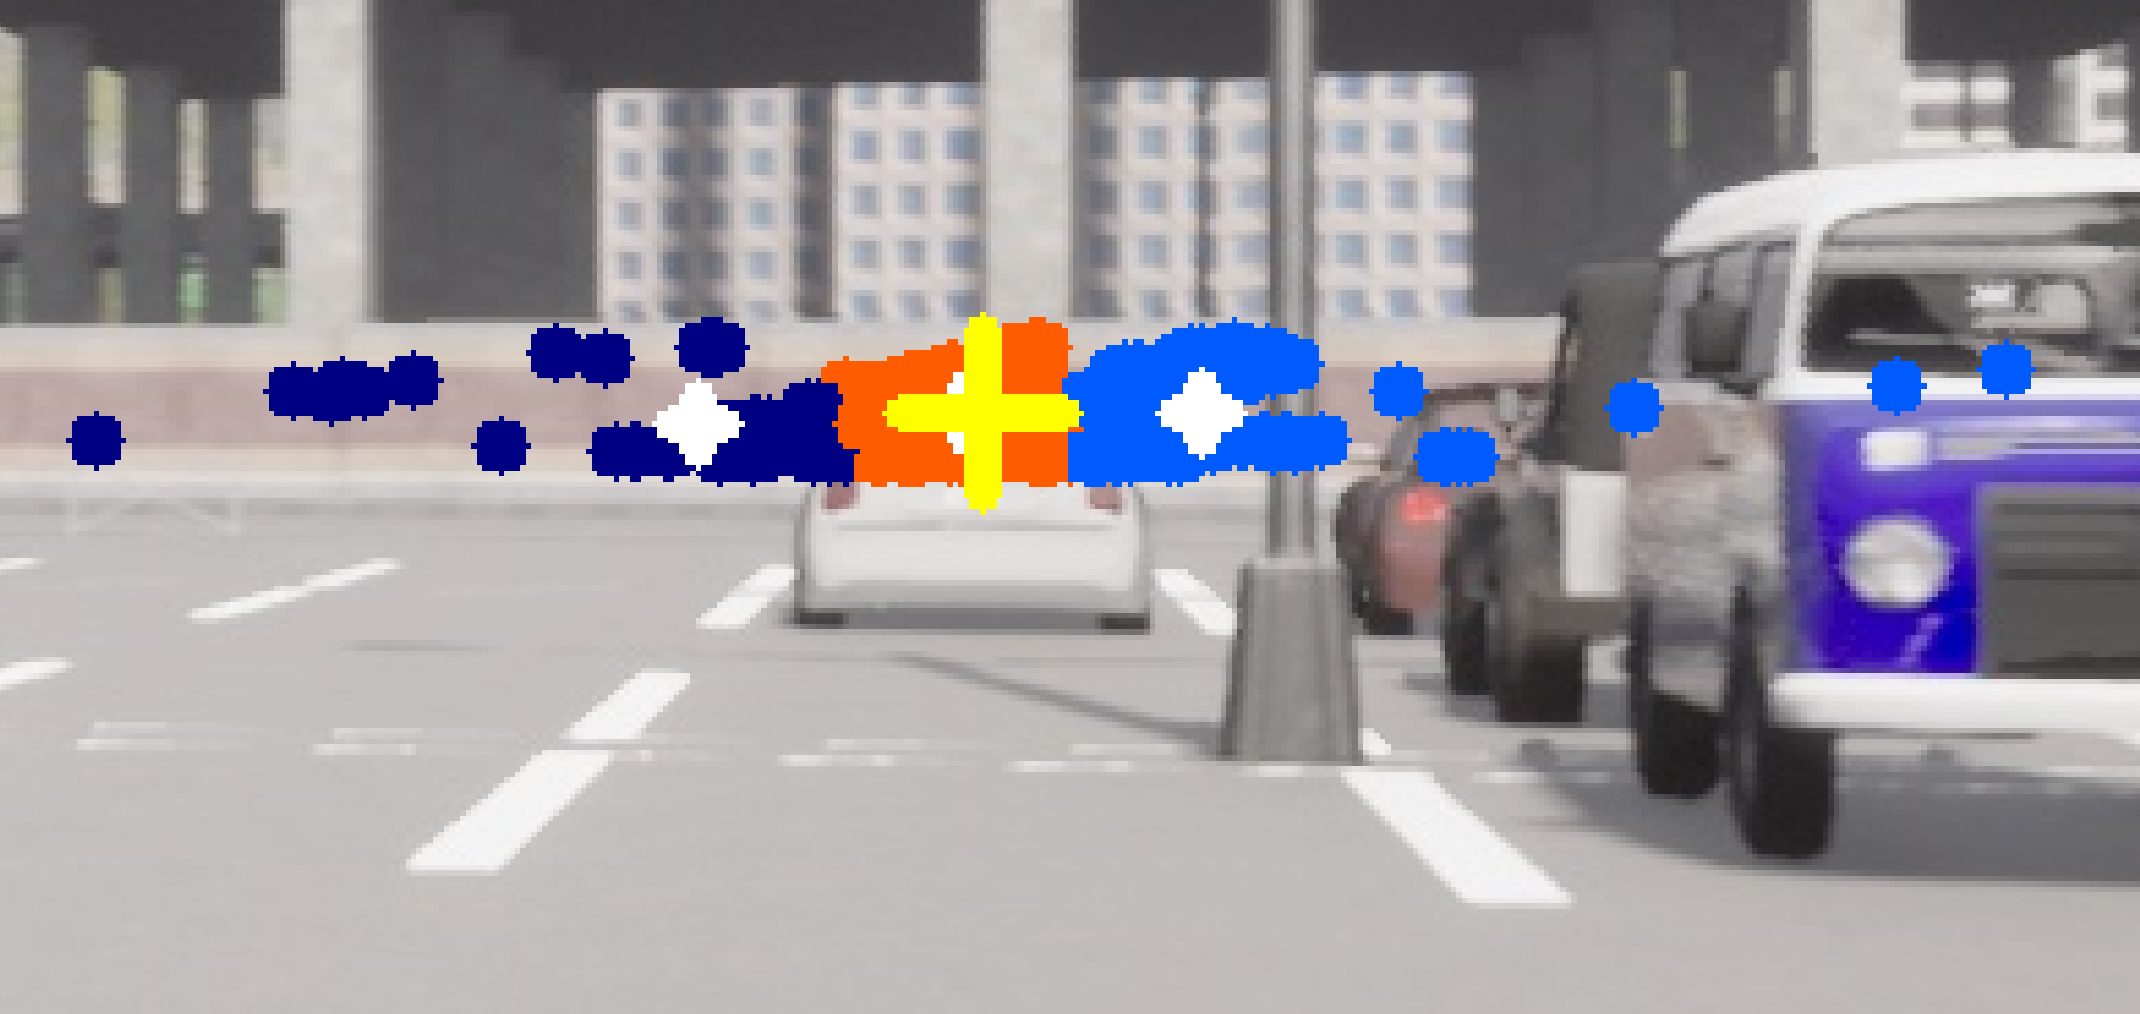
\includegraphics[width=0.8\textwidth]{img/reticule/vanishingPoint}
    \caption{Punto de fuga principal estimado}
    \label{fig:vanishingPoint}
\end{figure}

\subsubsection{Selección del 2do punto de fuga principal:}
Pendiente de redacción.

\subsubsection{Filtrado de intersecciones y líneas relevantes:}
\noindent
Una vez que se han identificado los puntos de fuga principales, se puede proceder a filtrar las intersecciones y las líneas que son
relevantes para la retícula de estacionamiento.
Primero, se filtran las intersecciones que están cerca de los puntos de fuga principales, utilizando un umbral de distancia que se puede ajustar experimentalmente.
Luego, se filtran las líneas que pasan por estas intersecciones relevantes.
Este proceso ayuda a eliminar el ruido y las líneas que no contribuyen a la formación de la retícula de estacionamiento.


\subsubsection{Ajuste de la retícula de estacionamiento utilizando (RANSAC):}
Pendiente de redacción (RANSAC).


\subsubsection{Experimentación y ajuste de parámetros:}\label{subsec:experimentacion-y-ajuste-de-parametros:}
\noindent
Para poder determinar la configuración óptima de los parámetros que se utilizan en los distintos algoritmos de la solución propuesta,
se desarrolló una aplicación en Python que carga una secuencia de imágenes de la trayectoria del vehículo en el estacionamiento y, para cada frame,
calcula la retícula de estacionamiento aplicando los pasos anteriormente descritos.
La aplicación permite visualizar los resultados de cada paso y ajustar dinámicamente los parámetros de los algoritmos para obtener los mejores resultados.
Los parámetros ajustables que se consideraron son:
\begin{itemize}
    \item \texttt{threshold\_image}: Umbral de binarización de la imagen.
    \item \texttt{canny\_threshold\_1}: Umbral inferior para el algoritmo de Canny.
    \item \texttt{canny\_threshold\_2}: Umbral superior para el algoritmo de Canny.
    \item \texttt{hough\_rho}: Resolución de la distancia en píxeles de la cuadrícula de la transformada de Hough.
    \item \texttt{hough\_theta}: Resolución del ángulo en radianes de la cuadrícula de la transformada de Hough.
    \item \texttt{hough\_threshold}: Umbral de votación de la transformada de Hough.
    \item \texttt{hough\_min\_line\_length}: Longitud mínima de la línea en píxeles.
    \item \texttt{hough\_max\_line\_gap}: Máxima separación entre segmentos de línea para tratarlos como una sola línea.
    \item \texttt{relevant\_intersections\_horizon\_threshold}: Umbral de cercanía al horizonte para considerar una intersección relevante.
    \item \texttt{agglomerative\_distance\_threshold}: Distancia máxima entre dos puntos para considerarlos en el mismo cluster.
\end{itemize}
Para analizar el impacto del cambio en los parámetros en tiempo real, la aplicación provee un menú de acciones que permite
representar en la imagen los resultados de cada paso del algoritmo.
%bloque de codigo
%\begin{lstlisting}[language=Python,label={lst:lstlisting22}]
%    --- Leyenda de Teclas ---
%P: Iniciar/Pausar la secuencia de imágenes.
%C: Mostrar/Ocultar contornos.
%L: Mostrar/Ocultar líneas.
%I: Mostrar/Ocultar intersecciones.
%R: Mostrar/Ocultar intersecciones relevantes.
%E: Mostrar/Ocultar líneas relevantes.
%A: Mostrar/Ocultar cúmulos de intersecciones.
%F: Mostrar/Ocultar puntos de fuga.
%G: Mostrar/Ocultar imagen binaria.
%ESC: Salir.
%\end{lstlisting}

\begin{verbatim}
    --- Leyenda de Teclas ---
P: Iniciar/Pausar la secuencia de imágenes.
C: Mostrar/Ocultar contornos.
L: Mostrar/Ocultar líneas.
I: Mostrar/Ocultar intersecciones.
R: Mostrar/Ocultar intersecciones relevantes.
E: Mostrar/Ocultar líneas relevantes.
A: Mostrar/Ocultar cúmulos de intersecciones.
F: Mostrar/Ocultar puntos de fuga.
G: Mostrar/Ocultar imagen binaria.
ESC: Salir.
\end{verbatim}
\noindent
A continuación, en las figuras \ref{fig:experimentationRgb} y \ref{fig:experimentationBinary} se muestra un ejemplo de la aplicación
en ejecución en uno de los frames de la secuencia de imágenes,
donde se visualizan los contornos, las líneas detectadas, las intersecciones, las intersecciones relevantes, las líneas relevantes,
los cúmulos de intersecciones y los puntos de fuga.

\begin{figure}[!ht]
    \begin{subfigure}{0.99\textwidth}
        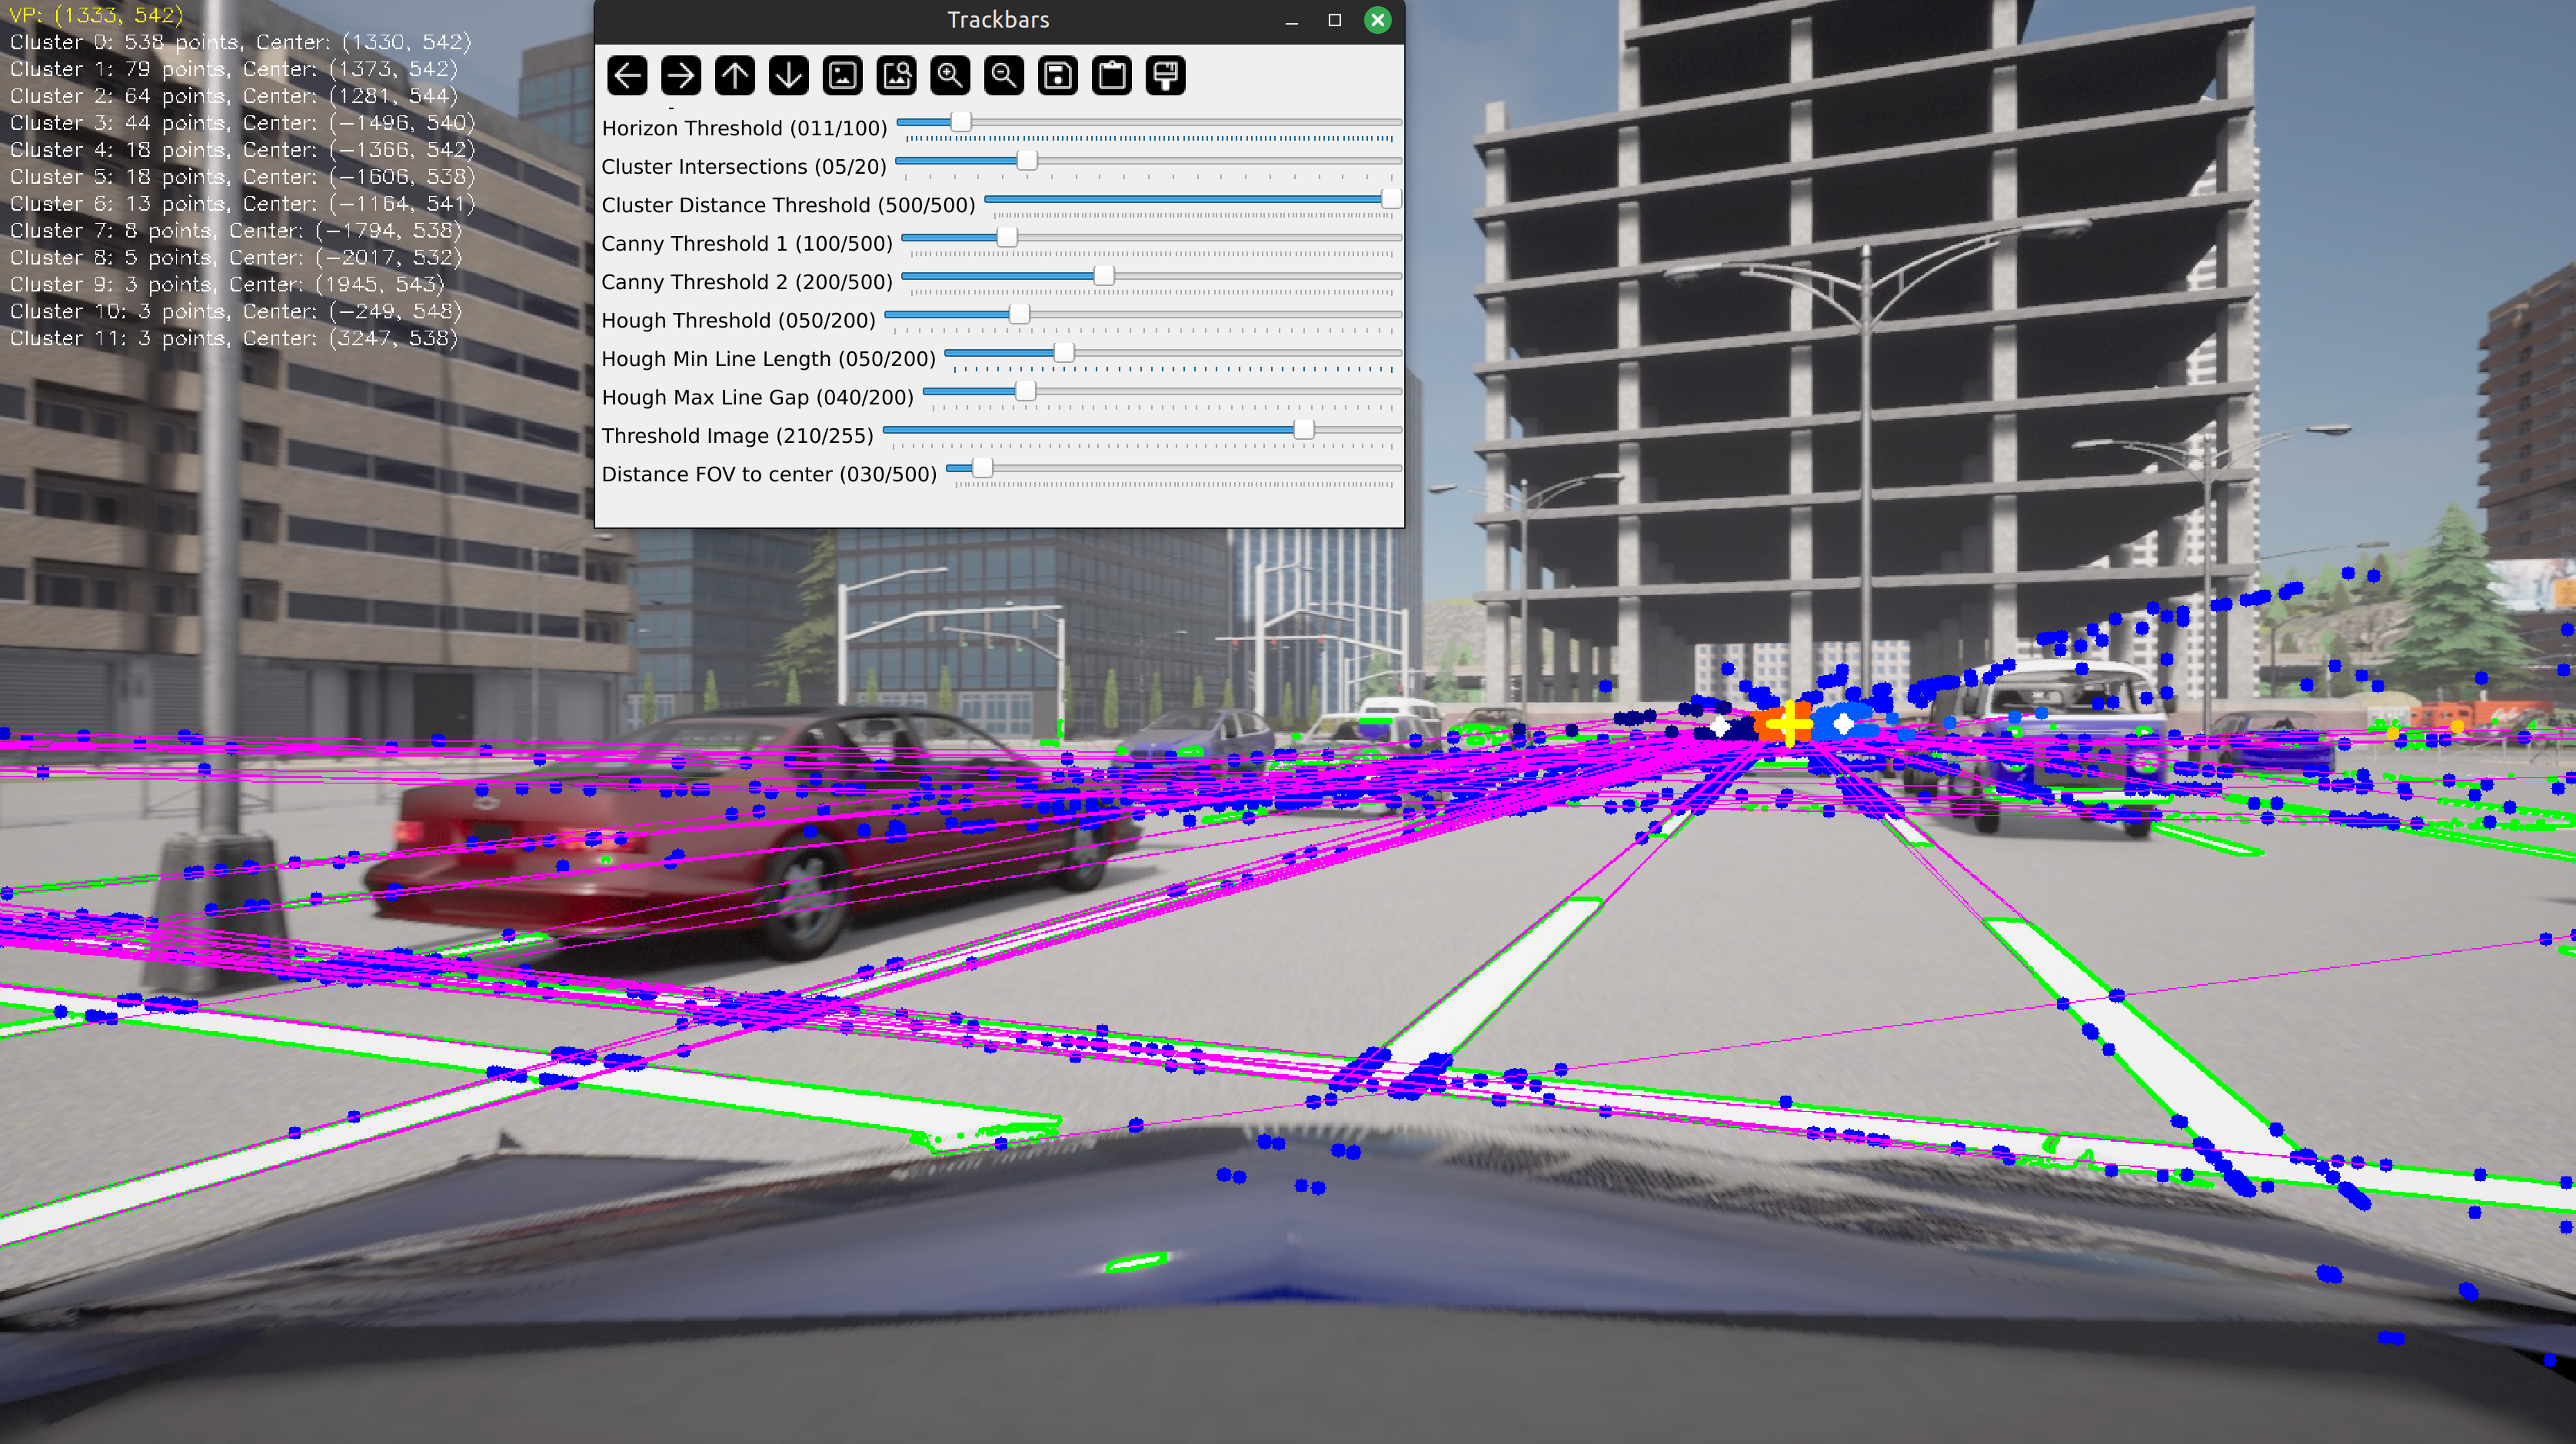
\includegraphics[width=\textwidth]{img/reticule/experimentationRgb}
        \caption{Ejemplo de experimentación (RGB)}
        \label{fig:experimentationRgb}
    \end{subfigure}
    \begin{subfigure}{0.99\textwidth}
        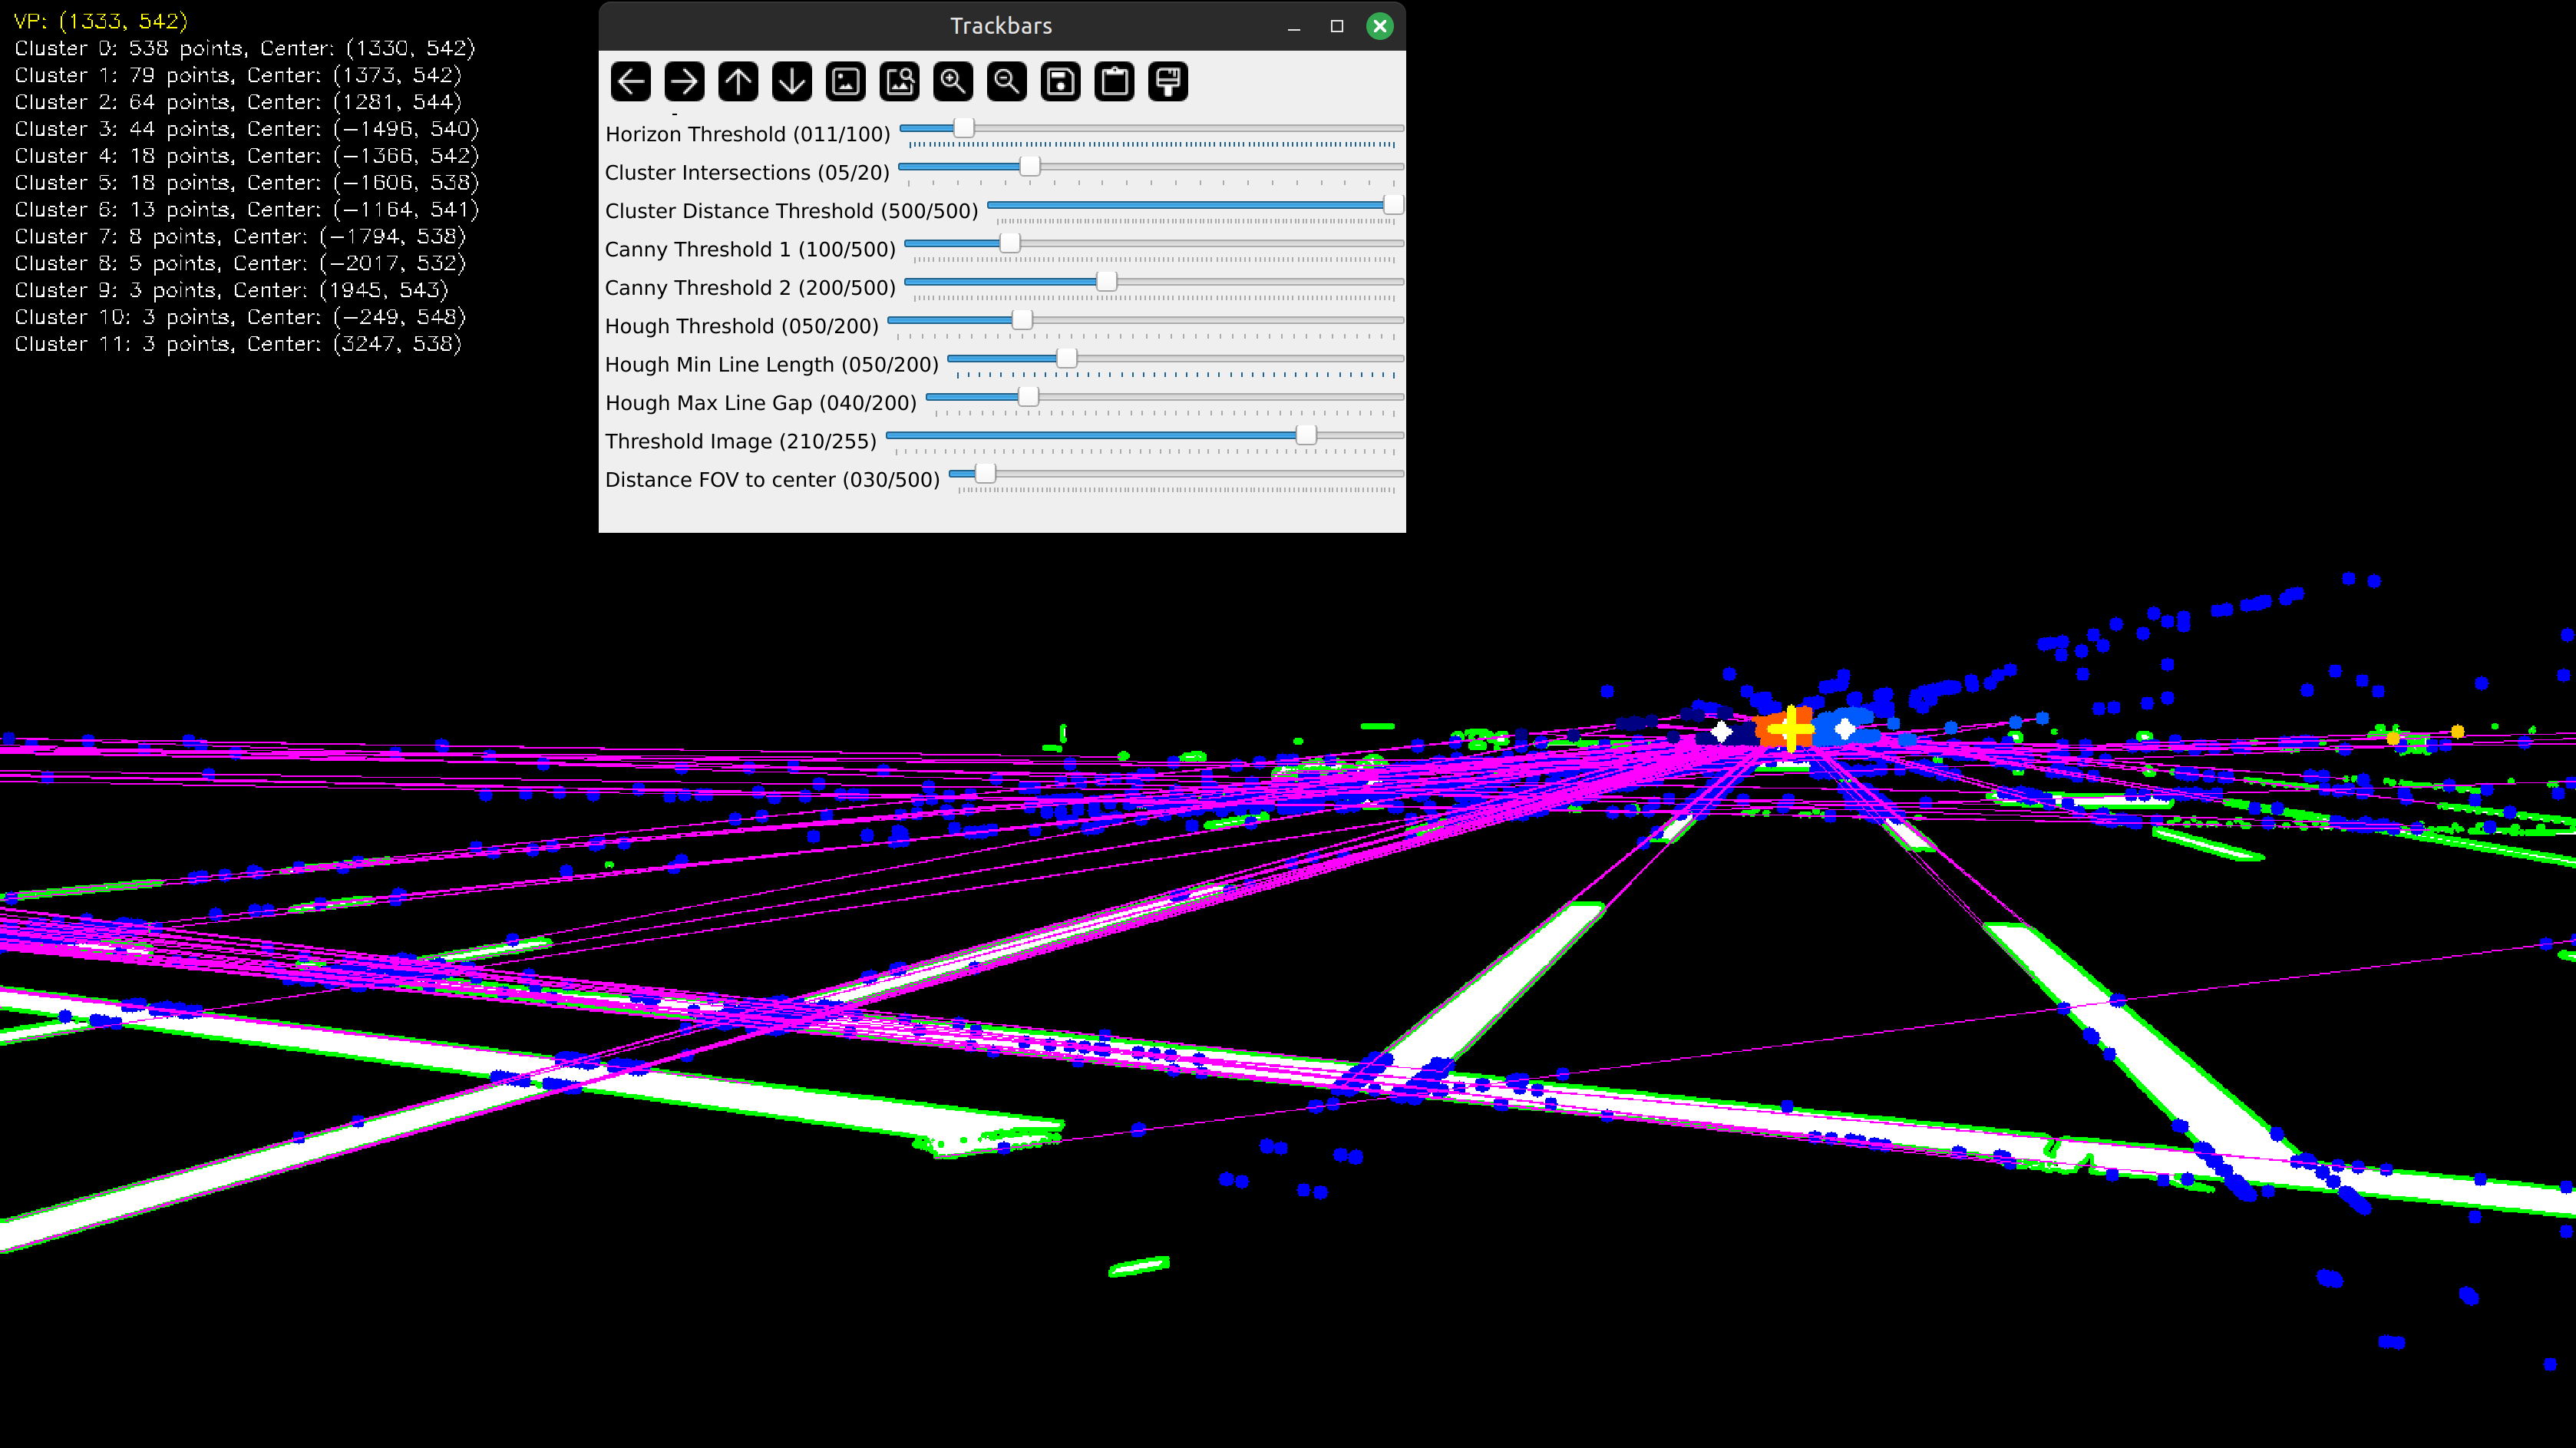
\includegraphics[width=\textwidth]{img/reticule/experimentationBinary}
        \caption{Ejemplo de experimentación (Binaria)}
        \label{fig:experimentationBinary}
    \end{subfigure}
\end{figure}

\noindent
Como se puede observar en la imagen, en el área de Trackbar se muestran los parámetros ajustables y su valor actual,
permitiendo al usuario modificarlos en tiempo real y observar el impacto de estos cambios en la imagen.
Esto facilita la identificación de la configuración óptima para cada parámetro, mejorando la precisión
y la robustez del algoritmo de detección de la retícula de estacionamiento.

\subsubsection{Mediciones en la retícula detectada:}
Pendiente de redacción.
